\documentclass[tikz,border=3pt]{standalone}
\usepackage[utf8]{inputenc}
\usepackage[T1]{fontenc}
\usepackage{lmodern}
\renewcommand{\familydefault}{\sfdefault}
\usepackage{sansmath}\sansmath
\usepackage[american]{circuitikz}
\usepackage{pgfplots}\pgfplotsset{compat=1.18,/pgf/number format/use comma,/pgf/number format/1000 sep={.}}
\usetikzlibrary{arrows.meta,calc,positioning,decorations.pathmorphing,patterns}
% paleta del sitio
\definecolor{nar}{HTML}{E8680C}\definecolor{narc}{HTML}{FFB35C}\definecolor{hielo}{HTML}{FFF3E8}
\definecolor{tinta}{HTML}{1D1D1F}\definecolor{gris}{HTML}{6E6E73}\definecolor{lila}{HTML}{7C5CF0}
\definecolor{azul}{HTML}{2F6FD6}\definecolor{menta}{HTML}{17A673}\definecolor{coral}{HTML}{E8342A}
\ctikzset{bipoles/thickness=1.6}
\begin{document}
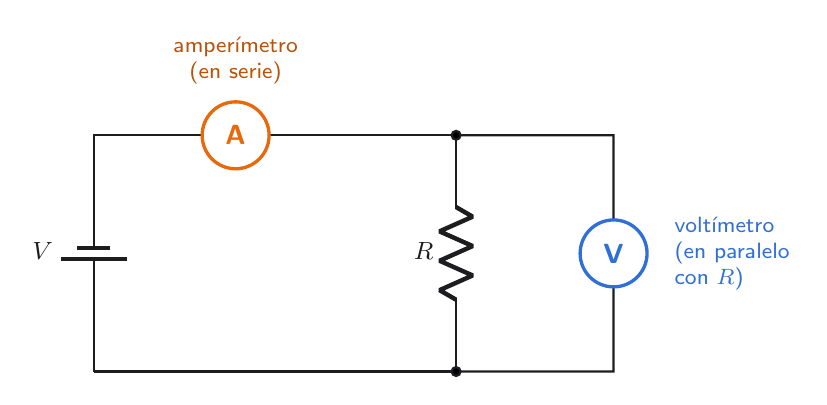
\begin{tikzpicture}[font=\small,>={Stealth[length=2.4mm]}]
\draw[tinta,thick] (0,0) to[battery1,l=$V$] (0,3) -- (4.6,3) to[R,l_=$R$] (4.6,0) -- (0,0);
\draw[tinta,thick] (4.6,3) to[short,*-] (6.6,3) -- (6.6,0) to[short,-*] (4.6,0);
\node[draw=nar,fill=white,very thick,circle,minimum size=0.85cm,font=\normalsize\bfseries,text=nar] at (1.8,3) {A};
\node[draw=azul,fill=white,very thick,circle,minimum size=0.85cm,font=\normalsize\bfseries,text=azul] at (6.6,1.5) {V};
\node[nar!80!black,font=\footnotesize,align=center] at (1.8,3.95) {amperímetro\\(en serie)};
\node[azul,font=\footnotesize,align=left,anchor=west] at (7.25,1.5) {voltímetro\\(en paralelo\\con $R$)};
\end{tikzpicture}
\end{document}
